\documentclass[a4paper]{article}

\usepackage{metalogo}
\usepackage{geometry}
\usepackage{indentfirst}
\usepackage{graphicx}
\usepackage{array}
\usepackage{booktabs}
\usepackage{listings}
\usepackage{color}
\usepackage{float}
\usepackage{tikz}
\usetikzlibrary{shapes.geometric, arrows, positioning}
\usepackage{textcomp}
\usepackage{chngcntr}
\usepackage{enumerate}
\usepackage{fancyhdr}
\usepackage{multirow}
\usepackage[colorlinks=false, pdfborder=0 0 0, bookmarksopen=true]{hyperref}
\usepackage{bookmark}
%\usepackage[backend=biber, style=numeric]{biblatex}
\usepackage[perpage]{footmisc}
\usepackage{setspace}
\usepackage{longtable}
\usepackage{arydshln}
\usepackage{amssymb}
\usepackage{amsmath}

% Other Settings %%%%%%%%%
%%%%%%%%%%%%%%%%%%%%%%%%%%
\geometry{left=1.2in, right=1.2in, top=1.2in, bottom=1.2in}
\renewcommand\thefigure{\Roman{section}-\arabic{subsection}-\arabic{figure}}
\renewcommand\thetable{\Roman{section}-\arabic{subsection}-\arabic{table}}
\counterwithin{figure}{section}
\counterwithin{figure}{subsection}
\setlength{\LTpre}{0pt}
\setlength{\LTpost}{0pt}



% Ctex Settings %%%%%%%%%%
%%%%%%%%%%%%%%%%%%%%%%%%%%
\usepackage[
fontset=none,		% a must-have option
heading=true,		% <true|false>		enable heading, affecet numbering
scheme=chinese,		% <chinese|plain>	use chinese scheme
linespread=1.3,		% line spreading
zihao=5				% set font size
]{ctex}

% this is an workaround for the wrong hyperref content
\newlength{\tempspacewidth}
\setlength{\tempspacewidth}{3em}

\ctexset{
	fontset=adobe,				% <adobe|fandol|founder|ubuntu|mac|windos|windowsnew|...>
	punct=quanjiao,				% <quanjian|banjiao|kaiming|plain>
	autoindent=true,			% <true|false|num|num-with-metric>
	today=small,				% <small|big|old> old for English format
	contentsname=目录,			% name of the content
	listfigurename=插图,		% name of listfigure
	listtablename=表格,			% name of the list table
	figurename=图,				% name of the figure
	tablename=表,				% name of the table
	indexname=索引,				% name of the index
	appendixname=附录,			% name of the appendix
	% --------------------------------------------
	% Whether parts's header should be numbered -- Number
	part/numbering=true,
	section/numbering=true,
	subsection/numbering=true,
	subsubsection/numbering=true,
	paragraph/numbering=true,
	subparagraph/numbering=true,
	appendix/numbering=true,
	% --------------------------------------------
	% Control the format of the NUMBERIG --------- Number
	section/name={,},					% section name, has the format of {AAA,BBB}
	subsection/name={,},
	subsubsection/name={,},
	appendix/name={附录},
	section/number=\Roman{section},		% can use \chinese{<counter>}
	subsection/number=\Roman{section}.\arabic{subsection},
	subsubsection/number=\Roman{section}.\arabic{subsection}.\arabic{subsubsection},
	paragraph/number=\arabic{paragraph},
	subparagraph/number=\arabic{paragraph}.\arabic{subparagraph},
	appendix/number=\Alph{section},
	% --------------------------------------------
	% Control the format of parts' header -------- Global
	section/format=\Large\bfseries,		% add \centering here if you want to centralize it
	subsection/format=\large\bfseries,
	subsubsection/format=\normalsize\bfseries,
	paragraph/format=\normalsize\bfseries,
	subparagraph/format=\normalsize\bfseries,
	% --------------------------------------------
	% Control the format of TOC ------------------ Name
	section/tocline=\Large\bfseries\CTEXnumberline{#1}#2,		% \CTEXnumberline means that if the section/etc has no name, then do not output the num
	subsection/tocline=\large\bfseries\CTEXnumberline{#1}#2,
	subsubsection/tocline=\normalsize\bfseries\CTEXnumberline{#1}#2,
	paragraph/tocline=\normalsize\CTEXnumberline{#1}#2,
	subparagraph/tocline=\normalsize\CTEXnumberline{#1}#2,
}



% Definitions %%%%%%%%%%%%
%%%%%%%%%%%%%%%%%%%%%%%%%%

\newcommand{\coverpage}{
	\thispagestyle{empty}
	\pagenumbering{gobble}
}

\newcommand{\toc}{
	\newpage
	\pagenumbering{Roman}
	\setcounter{page}{1}
	\tableofcontents
}

\newcommand{\maincontents}{
	\newpage
	\pagestyle{fancy}
	\setlength{\headheight}{12.2pt}
	\setlength{\headsep}{15pt}
	\pagenumbering{arabic}
	\setcounter{page}{1}
}

\lstset{language=[x86masm]Assembler,
		tabsize=4,
		breaklines=true,
		frame=shadowbox,
		framexleftmargin=7mm,
		rulesepcolor=\color{black},
		basicstyle=\footnotesize,
		numbers=left,
		showspaces=false,
		showstringspaces=false
}
\newfontfamily\codeF{Courier New}
\newfontfamily\codeI{monofur}
\newenvironment{codeFont}{\codeF}{\par}
\newenvironment{codeInteresting}{\codeI}{\par}


% Starting the main contents %%%%%%%%%%%
%%%%%%%%%%%%%%%%%%%%%%%%%%%%%%%%%%%%%%%%
%%%%%%%%%%%%%%%%%%%%%%%%%%%%%%%%%%%%%%%%
%%%%%%%%%%%%%%%%%%%%%%%%%%%%%%%%%%%%%%%%
\begin{document}

% cover page %%%%%%%%%%%%%%%%%%%
%%%%%%%%%%%%%%%%%%%%%%%%%%%%%%%%
\coverpage

\ \\ \vspace{1cm}

\begin{flushleft}
	\begin{tabular}{c}
		{\Huge 
\includegraphics[width = 10em]{resources/hust.jpg}} \\
		{\fangsong \textbf{\Huge \makebox[9em][s]{课程实验报告}}} \\[0.6cm]
		{\fangsong {\Large 课程名称:\underline{计算机系统基础}}}
	\end{tabular}
\end{flushleft}

\vfill

\begin{flushright}
	\begin{tabular}{r m{8em}}
		\makebox[6em][s]{专业班级:} & 计卓1501 \\ \cline{2-2}
		\makebox[6em][s]{学号:} & U201514898 \\ \cline{2-2}
		\makebox[6em][s]{姓名:} & 胡思勖 \\ \cline{2-2}
		\makebox[6em][s]{指导教师:} & 谭志虎 \\ \cline{2-2}
		\makebox[6em][s]{报告日期:} & 2017年6月1日 \\ \cline{2-2}
	\end{tabular}
\end{flushright}

\vspace{3cm}

% table of contents %%%%%%%%%%%%
%%%%%%%%%%%%%%%%%%%%%%%%%%%%%%%%
\toc

% main contents %%%%%%%%%%%%%%%%
%%%%%%%%%%%%%%%%%%%%%%%%%%%%%%%%
\maincontents
\section{实验概述}
\subsection{实验目标、要求}
本实验中,你要使用课程所学知识拆除一个“binary bombs”。一个“binary bombs”(二进制炸弹,下文将简称为炸弹)是一个 Linux 可执行C 程序,包含了 6 个阶段(phase1~phase6)。炸弹运行的每个阶段要求你输入一个特定的字符串,若你的输入符合程序预期的输入,该阶段的炸弹就被“拆除”,否则炸弹“爆炸”并打印输出 "BOOM!!!"字样。实验的目标是拆除尽可能多的炸弹层次。六个层次如下:
\begin{itemize}
	\item 阶段 1:字符串比较
	\item 阶段 2:循环
	\item 阶段 3:条件/分支
	\item 阶段 4:递归调用和栈
	\item 阶段 5:指针
	\item 阶段 6:链表/指针/结构
	\item 隐藏阶段: 只有当你在第 4 阶段的解之后附加一特定字符串后才会出现。
\end{itemize}

\subsection{实验意义}
本实验用于增强对程序的机器级表示、汇编语言、调试器和逆向工程等方面原理与技能的掌握。\par

% Phases %%%%%%%%%%%%%%%%%%%%%%%
%%%%%%%%%%%%%%%%%%%%%%%%%%%%%%%%
\newpage
\section{内容}

\subsection{阶段1}
\subsubsection{任务描述}
第一阶段主要检测反汇编中的基础部分,通过对于字符串比较过程的解析来拆除炸弹的第一阶段。

\subsubsection{实验过程}
\begin{itemize}
	\item 首先,对于程序进行反汇编,观察主程序入口的反汇编结果,发现第一阶段调用的为phase\_1函数。此外,还发现第n个阶段调用的为phase\_<n>函数。在每个函数调用完毕后,调用phase\_defused函数。由此可以推测,第一阶段的主要任务是分析phase\_1的内容。
	\item 跳转到phase\_1的部分,发现其反汇编代码如下:
		\begin{codeFont}
			\lstinputlisting{resources/code1.asm}
		\end{codeFont}
	\item 发现此函数调用了strings\_not\_equal子过程。而为string\_not\_equal子过程传入的参数一个为phase\_1的传如参数,另一为常量地址0x804a324。
	\item 根据函数名称和传入参数可以推测,此函数即为将传入字符串与一固定字符串进行比较,且0x804a324处即为此常量字符串。
	\item 对于bomb二进制文件从0x804a324处进行反汇编,如图\ref{fig:fig1}所示。
		\begin{figure}[H]
			\centering
			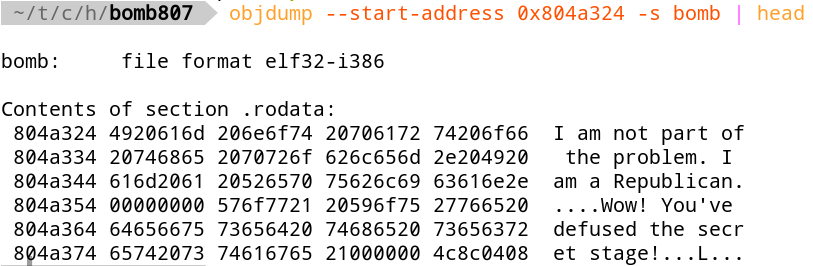
\includegraphics[width=0.95\linewidth]{resources/fig1.png}
			\caption{bomb从0x804a324的反汇编内容}
			\label{fig:fig1}
		\end{figure}
	\item 由此可以看出,此固定字符串的内容为``I am not part of the problem. I am a Republican.''
	\item 将此字符串输入bomb程序,第一阶段成功解除,如图\ref{fig:fig2}所示。
		\begin{figure}[H]
			\centering
			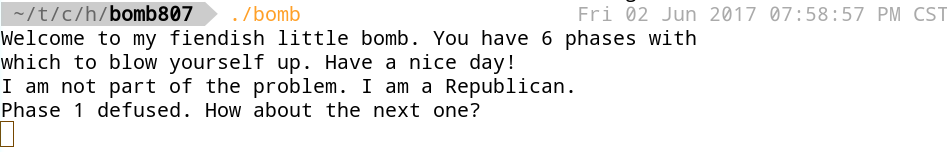
\includegraphics[width=0.95\linewidth]{resources/fig2.png}
			\caption{第一阶段解除}
			\label{fig:fig2}
		\end{figure}
\end{itemize}

\subsubsection{实验结果}
由实验过程可知,第一阶段的解为字符串``I am not part of the problem. I am a Republican.'',第一阶段成果解除。

\subsection{阶段2}
\subsubsection{任务描述}
阶段二需要我们通过对于汇编中循环的分析来解析程序,从而推测这一阶段的解。

\subsubsection{实验过程}
\begin{itemize}
	\item 由第一阶段可知,第二阶段应该从phase\_2开始。
	\item 在反汇编中跳转到phase\_2的部分,反汇编代码如下(已添加必要注释):
		\begin{codeFont}
			\lstinputlisting{resources/code2.asm}
		\end{codeFont}
	\item 从代码中可以看出,在0x8048bc8处调用了read\_six\_numbers函数,从函数名推测,应该需要读入六个整数。其中parameter注释部分为read\_six\_numbers的实参。
	\item 在读入六个整数后,将第一个整数与\$0x1进行比较,如果不相等则炸弹爆炸,因此推断出第一个整数为1。
	\item 对于接下来的标签的分析,可以发现其为一个do-while型循环,初始化esi为读入六个字符数组的超尾地址,ebi 数组的第二个元素,每次ebi向后移动一个整型大小,直到循环完整个数组为止。
	\item 在循环体(0x8048bdb - 8048be4)中,从第二个元素开始,将每一个元素与前一个元素进行比较,如果不为前一个元素的两倍则炸弹爆炸,因此推测第二个炸弹的解为一个等比数列,且初始值为1,因此解为``1 2 4 8 16 32''。
	\item 输入炸弹,成功拆除第二层,如图\ref{fig:fig3}所示。
		\begin{figure}[H]
			\centering
			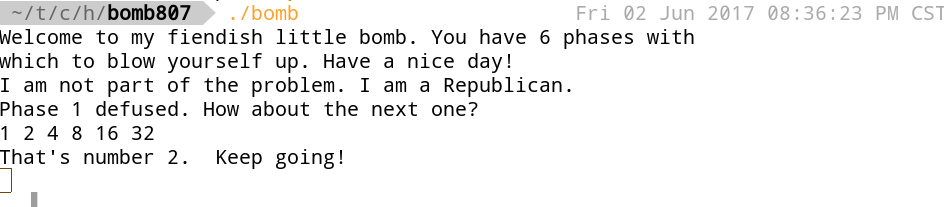
\includegraphics[width=0.95\linewidth]{resources/fig3.png}
			\caption{第二阶段炸弹拆除}
			\label{fig:fig3}
		\end{figure}
\end{itemize}

\subsubsection{实验结果}
第二阶段的解为字符串``1 2 4 8 16 32''。

\subsection{阶段3}
\subsubsection{任务描述}
阶段三考察对于条件与分支判断的汇编语言解析,需要通过解析汇编条件判断的结构来拆除第三层。

\subsubsection{实验过程}
\begin{itemize}
	\item 在反汇编中跳转到phase\_3的部分,反汇编代码如下(已添加必要注释):
		\begin{codeFont}
			\lstinputlisting{resources/code3.asm}
		\end{codeFont}
	\item 可以看出,首先调用了sscanf函数,且sscanf函数的第二个参数(格式化字符串)为一常量字符串,且存储在0x804a5b1处。通过从这一地址开始反汇编,可以得到格式化字符串为``\%d \%d'',如图\ref{fig:fig4}所示。
		\begin{figure}[H]
			\centering
			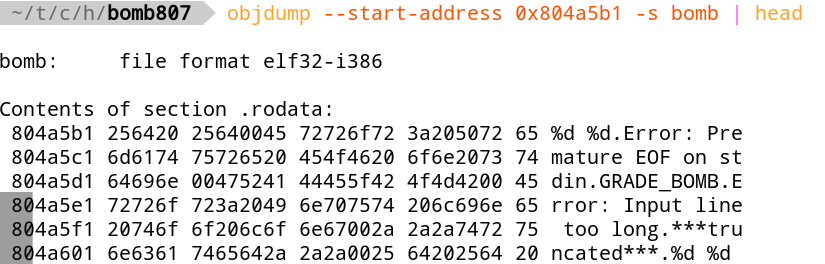
\includegraphics[width=0.95\linewidth]{resources/fig4.png}
			\caption{格式化字符串的反汇编}
			\label{fig:fig4}
		\end{figure}
	\item 在反汇编之后,将读入的第一个数与\$0x7比较(0x8048c33处),若比7大则炸弹爆炸,说明第一个数比7小。
	\item 观察到后面的程序进行了一系列的跳转,较为难以进行静态分析,因此直接打开GDB调试。在命令行中输入gdb bomb后,在0x8048c3a处打上断点,将前两题的答案写入result.txt中,然后在gdb中输入r result.txt;
	\item 进入第三阶段后,输入``1 1'',然后单步执行观察程序运行状态。如图\ref{fig:fig5}所示。
		\begin{figure}[H]
			\centering
			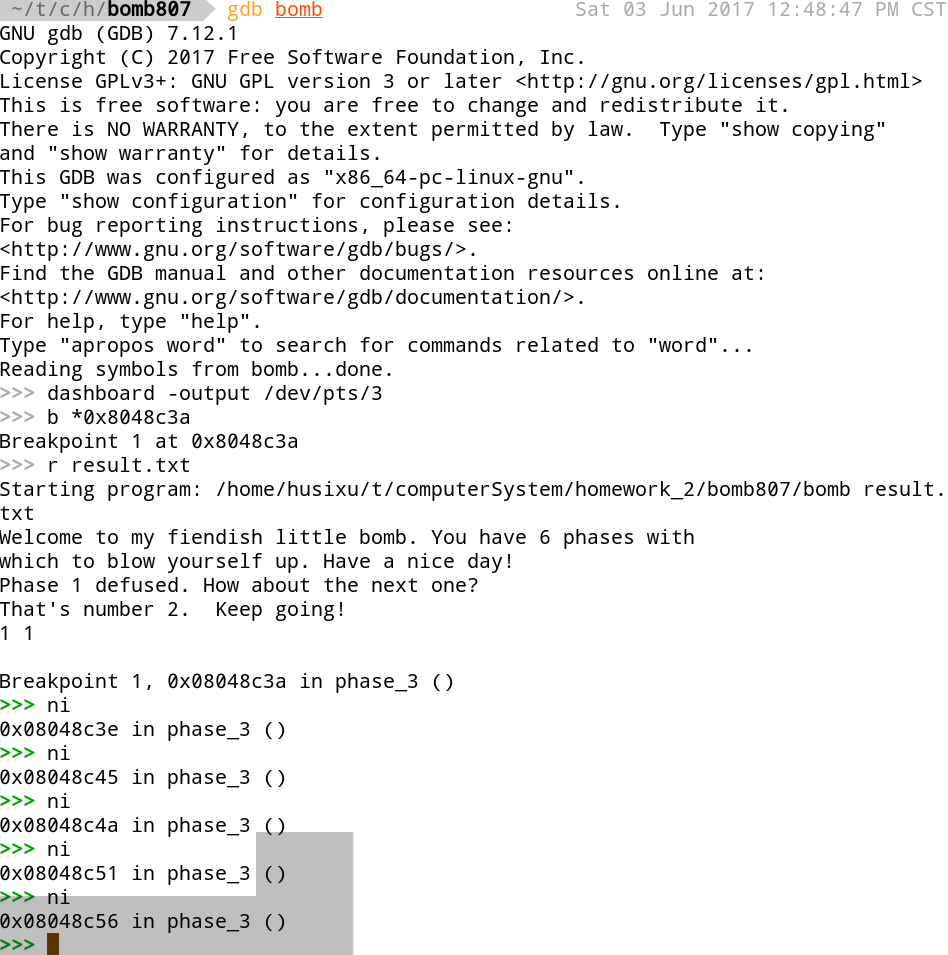
\includegraphics[width=0.95\linewidth]{resources/fig5.png}
			\caption{进入gdb调试}
			\label{fig:fig5}
		\end{figure}
	\item 发现单步执行一段时间后,发现执行到了0x8048caa处,首先将scanf获得的第一个数字与\$0x5比较,若大于5则跳转到炸弹爆炸位置,然后将eax中的内容与scanf获得的第二个数字比较,如果相等则结束程序,否则炸弹爆炸。而输入的第一个参数为1,满足小于5的条件,因此只要保证运行到此处时第二个参数与\%eax中的内容相等即可。
	\item 根据调试信息,此时\%eax中的内容为0xfffffe27,如图\ref{fig:fig6}所示,转化为10进制为-473。由此断定第二个数为-473。
		\begin{figure}[H]
			\centering
			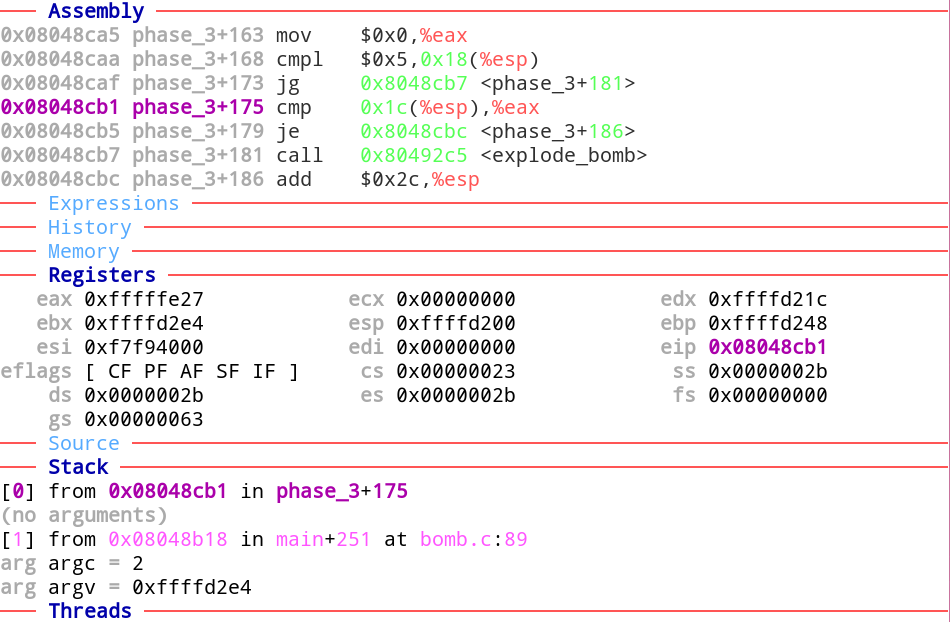
\includegraphics[width=0.95\linewidth]{resources/fig6.png}
			\caption{\%eax中的内容}
			\label{fig:fig6}
		\end{figure}
	\item 退出gdb,将第阶段的结果写入result.txt执行bomb result.txt,第阶段成功解除。如图\ref{fig:fig7}所示。
		\begin{figure}[H]
			\centering
			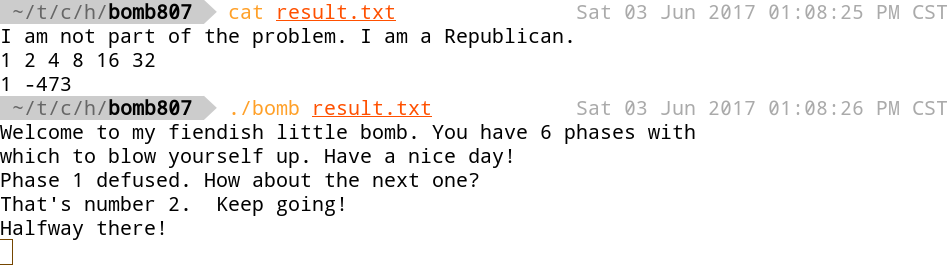
\includegraphics[width=0.95\linewidth]{resources/fig7.png}
			\caption{第三阶段解除}
			\label{fig:fig7}
		\end{figure}
\end{itemize}

\subsubsection{实验结果}
第三阶段的解为字符串``1 2 4 8 16 32'',第三阶段成功拆除。

\subsection{阶段4}
\subsubsection{任务描述}
第四阶段要求对递归调用的分析完成,由于涉及到栈的动态变化,这一阶段较为困难。

\subsubsection{实验过程}
\begin{itemize}
	\item 在反汇编中跳转到phase\_4的部分,反汇编代码如下(已添加必要注释):
		\begin{codeFont}
			\lstinputlisting{resources/code4.asm}
		\end{codeFont}
	\item 可以看出,程序执行了一次scanf,并且第二个实参与phase\_3中的实参一样,古这一阶段也要求输入两个整数。
	\item 在读入数字后,首先将第一个熟悉与\$0xe进行比较(0x8048d4e处),并且要求第一个参数小于或等于0xe,否则炸弹爆炸。
	\item 然后调用了func4子程序,传入的参数依次为scanf获得的第一个数字、0、0xe。
	\item 在调用完毕后,首先将返回值与\$0x6比较(0x8048d76处),要求返回值等于6,然后将scanf获得的第二个参数与0x6相比较(0x8048d7b处),也要求相等。而在调用func4时未传入scanf获得的第二个参数,因此推测scanf获得的第二个参数不变,为6。
	\item 对于func4进行分析,得到func4的流程图如图\ref{fig:fig8}所示。
		\begin{figure}[H]
			\centering
			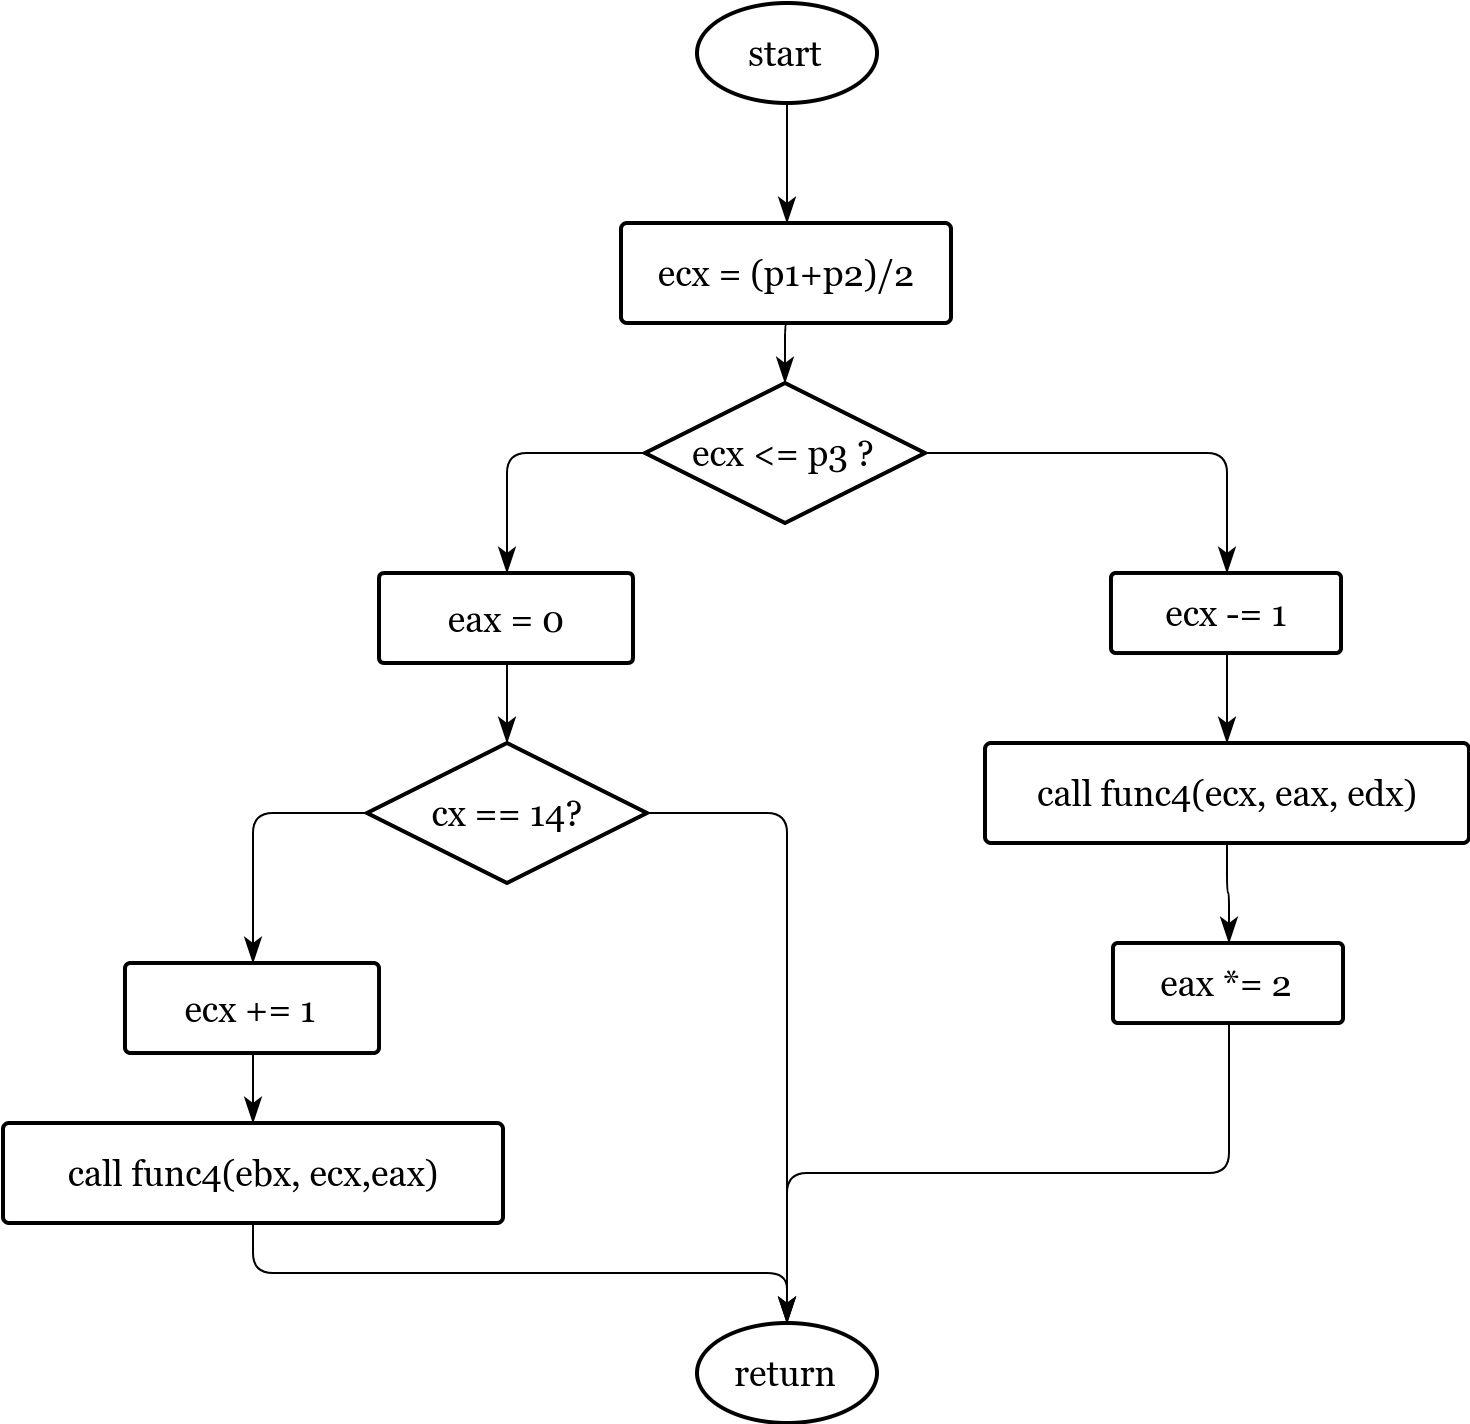
\includegraphics[width=0.95\linewidth]{resources/fig8.png}
			\caption{func4流程图}
			\label{fig:fig8}
		\end{figure}
	\item 由于func4的流程过于复杂,且带有递归,因此分析起来较为困难,故放弃分析。但是由phase4的已知条件可以知道第一个参数小于14,第二个参数为6,因此直接使用暴力手段进行拆解:从0开始对第一个参数逐个进行尝试,运行到0x804d76处观察func4的返回值是否为6,若不为6,则强制结束程序并使用下一个整数进行测试,直到测试的返回值为6为止。
	\item 通过上述测试,发现参数1的值为6。图\ref{fig:fig9}展示了第四阶段拆除后的结果。
		\begin{figure}[H]
			\centering
			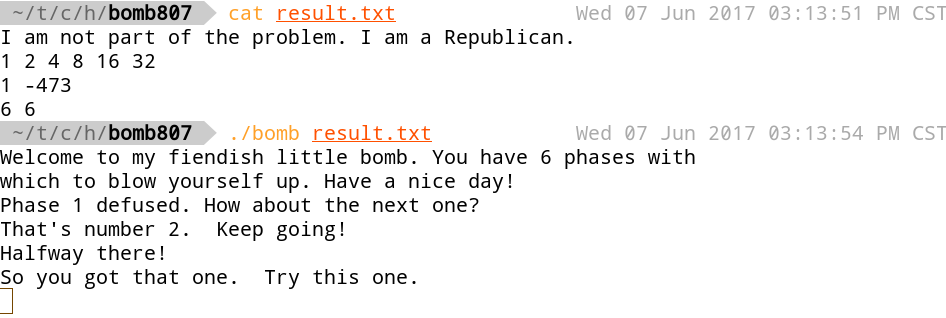
\includegraphics[width=0.95\linewidth]{resources/fig9.png}
			\caption{第四阶段拆除}
			\label{fig:fig9}
		\end{figure}
\end{itemize}

\subsubsection{实验结果}

\subsection{阶段5}
\subsubsection{任务描述}
第五阶段最要考察对于指针的分析。通过分析汇编代码语句对应的C语言指针操作来对炸弹进行拆除。

\subsubsection{实验过程}
\begin{itemize}
	\item 首先跳转到phase\_5的代码处,代码如下:
		\begin{codeFont}
			\lstinputlisting{resources/code5.asm}
		\end{codeFont}
	\item 对于汇编代码进行分析,发现首先调用了sscanf函数,且读入的格式化字符串地址与第三、第四阶段相同,均为0x804a5b1,因此可以断定这一阶段的答案为两个整数。
	\item 对于接下来的代码进行分析,发现器为一个简单的循环。循环的出事条件为\%eax = <第一个参数>\&0xf(0x8048dc0处),结束条件为\%eax为15(0x8048de2处)。在这些循环中,每次去以0x804a3a0为数组首地址,以eax为索引的一个数(0x8048dd9处),并存入eax中。并且,每次循环中edx+=1(0x8048dd6处),ecx+=<取出的数>(0x8048de0处)。
	\item 通过对跳出循环后的语句的分析,可以看到要求最后edx必须为15(ox8048deb处),且ecx必须与scanf读入的第二个数相等。由此可以推断,第一个参数需要保证循环体恰好循环15次,且最后一次取出的值为0xf,第二个参数则是取出的所有值的和。
	\item 对于循环中出现的数组进行反汇编,得到数组中的值依次为0xa, 0x2, 0xe, 0x7, 0x8, 0xc, 0xf, 0xb, 0x0, 0x4, 0x1, 0xd, 0x3, 0x9, 0x6, 0x5,如图\ref{fig:fig10}所示。
	\begin{figure}[H]
		\centering
		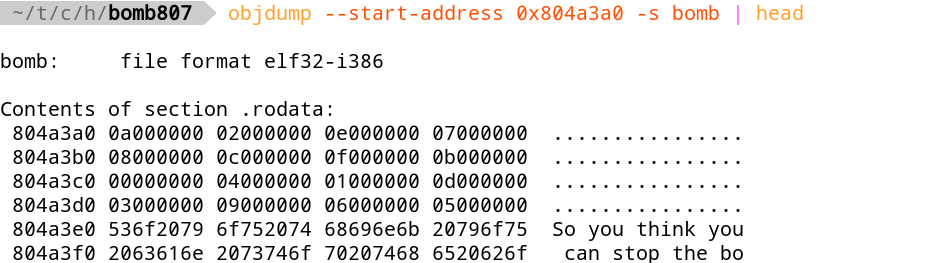
\includegraphics[width=0.95\linewidth]{resources/fig10.png}
		\caption{对于数组的反汇编}
		\label{fig:fig10}
	\end{figure}
	得到次数组后按照所得的规则进行逆推,得到第一个参数为5,第二个参数为115。输入炸弹,炸弹的第五阶段成功被拆除,如图\ref{fig:fig11}所示。
	\begin{figure}[H]
		\centering
		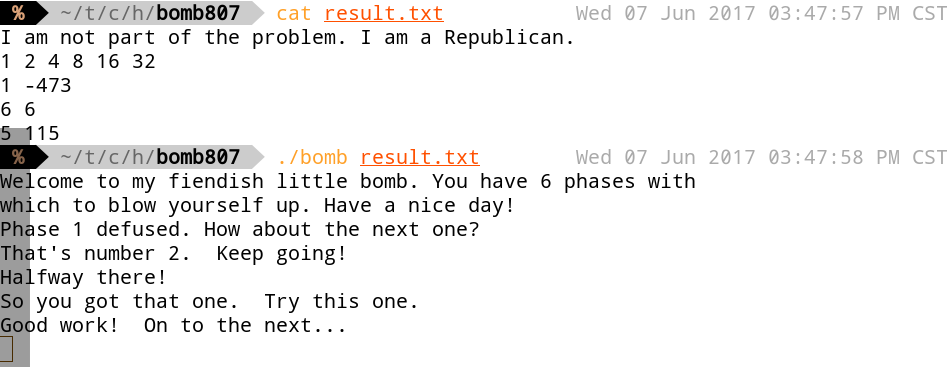
\includegraphics[width=0.95\linewidth]{resources/fig11.png}
		\caption{第五阶段拆除成功}
		\label{fig:fig11}
	\end{figure}
\end{itemize}

\subsubsection{实验结果}
第五阶段的解为字符串``5 115''

\subsection{阶段6}
\subsubsection{任务描述}
实验六较为复杂,要求通过对于汇编代码中的结构/链表操作进行分析并得出第六阶段的结果,对于结构体在内存中的存储方式进行了考察。

\subsubsection{实验过程}
\begin{itemize}
	\item 首先跳转到phase\_6的位置,代码如下(由于phase\_6的代码较长,因此分析时加入了较多的注释,===>为在这一部分推断出的的限制条件):
		\begin{codeFont}
			\lstinputlisting{resources/code4.asm}
		\end{codeFont}
	\item 首先,粗略的对于代码进行分段,将代码分为五个部分(注释中的part1~part5)并逐个进行分析。
	\item 第一部分:
		\begin{itemize}
			\item 调用read\_six\_numbers 读入六个数字。
				进行循环,将每一个数减一以后与5进行比较,要求$\leqslant 5$,推断出读入的六个数中每一个都$\leqslant 6$。
				进行第二个循环,这是一个二重循环,检测每一个数是否相等,如果不相等则炸弹爆炸,推测出读入的六个数两两不相等。
		\end{itemize}
	\item 第二部分:
		\begin{itemize}
			\item 进行一个循环,对于读入的每一个数进行处理,将7-<读入的数>存入一个数组的对应位置中,此列表在栈空间中并与读入的六个数的位置紧邻。
		\end{itemize}
	\item 第三部分:
		\begin{itemize}
			\item 这一部分较为复杂,也是较为重要的一部分。首先对其进行观察,发现它涉及到地址0x804c154,从这个地址开始反汇编,结果如图\ref{fig:fig12}所示。
				\begin{figure}[H]
					\centering
					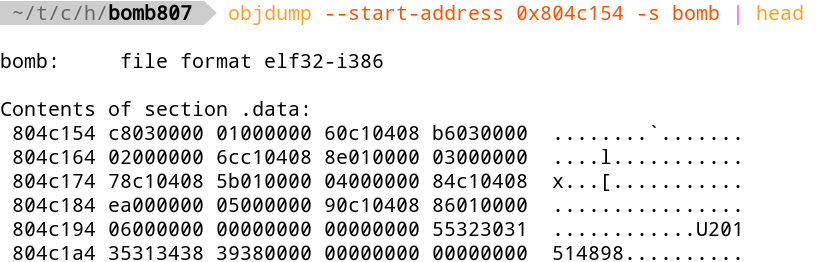
\includegraphics[width=0.95\linewidth]{resources/fig12.png}
					\caption{对于0x804c154的反汇编}
					\label{fig:fig12}
				\end{figure}
			\item 显然,这是一个链表,链表中的每一个节点为一个结构,占12个字节,且第三个成员为next指针。
			\item 经过分析后发现,这一部分进行的操作为对第二部分中的数组中的元素进行赋值。赋值规则为tab[i+6] = chain + i,其中chain为链表的首地址。
		\end{itemize}
	\item 第四部分:对于第三部分的排序后的链表进行了重新的链接。
	\item 第五部分:对于重新链接的链表进行了检查,要求保证链表从首至尾是升序有序的。
		整合上面的信息,输入的数据应该是对于原链表中的数据0x3c8, 0x3b6, 0x18e, 0x15b, 0xea, 0x186 进行排序,并用7减去排序后的索引,然后进行倒序的结果。推算出应为6 5 4 1 3 2,将``6 5 4 1 3 2''输入炸弹,成功拆除,如图\ref{fig:fig13}所示。
		\begin{figure}[H]
			\centering
			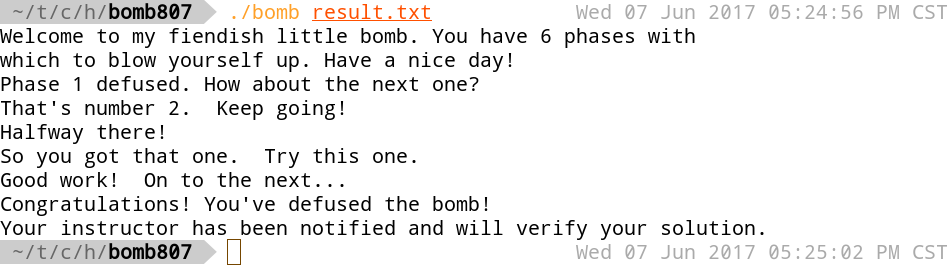
\includegraphics[width=0.95\linewidth]{resources/fig13.png}
			\caption{第六阶段成功拆除}
			\label{fig:fig13}
		\end{figure}
\end{itemize}

\subsubsection{实验结果}
第六阶段的解为字符串``6 5 4 1 3 2''

\subsection{隐藏阶段}
\subsubsection{任务描述}
找到如何进入隐藏阶段并对于隐藏阶段的炸弹进行拆解。

\subsubsection{实验过程}
\begin{itemize}
	\item 在反汇编代码中全文搜索phase时,发现了secrect\_phase函数,根据名称即可推测此为隐藏阶段,然后全文搜索其地址8048f3e,发现其入口在phase\_defused中。两个函数的反汇编代码如下。
		\begin{itemize}
			\item phase\_defused函数:
				\begin{codeFont}
					\lstinputlisting{resources/code7_1.asm}
				\end{codeFont}
			\item secrect\_phase函数:
				\begin{codeFont}
					\lstinputlisting{resources/code7_2.asm}
				\end{codeFont}
		\end{itemize}
	\item 首先对于phase\_defused进行分析,发现其strings\_not\_equal函数的一个参数为地址0x804a614。对于bomb进行反汇编,发现此处的字符串为DrEvil,因此推测,进入隐藏阶段的字符串为DrEvil。根据提示将起附加在phase\_4的解后面,成功进入隐藏阶段,如图\ref{fig:fig14}所示。
		\begin{figure}[H]
			\centering
			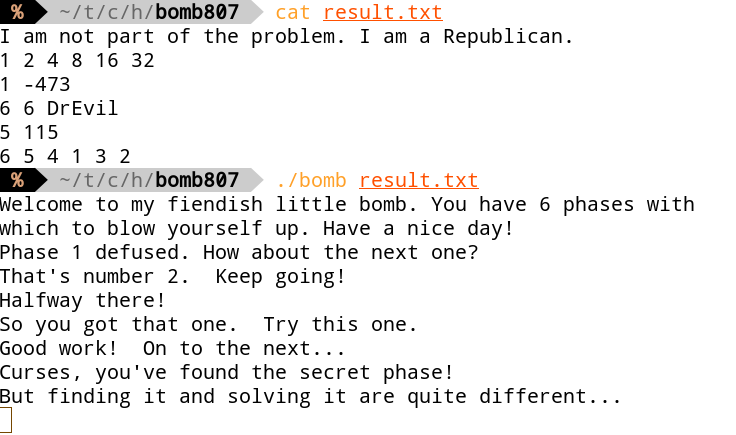
\includegraphics[width=0.95\linewidth]{resources/fig14.png}
			\caption{进入隐藏阶段}
			\label{fig:fig14}
		\end{figure}
	\item 然后对于隐藏阶段的代码进行分析,发现首先读入一个字符串,然后将字符串按照10进制转换为长整形,并将这一长整形作为fun7的参数并调用fun7。然后要求fun7的返回值为0。其中fun7的反汇编代码如下:
		\begin{codeFont}
			\lstinputlisting{resources/code7_3.asm}
		\end{codeFont}
	\item 对于fun7进行分析,发现其对存在于0x804c0a0(作为参数传入fun7)的二叉树进行搜索,二叉树反汇编图\ref{fig:fig15}所示,在其中查找隐藏阶段的解的位置,然后进行回溯,若回溯的边链接的是左子树,则返回值乘以2,若为右子树则乘以2再加上1。
		\begin{figure}[H]
			\centering
			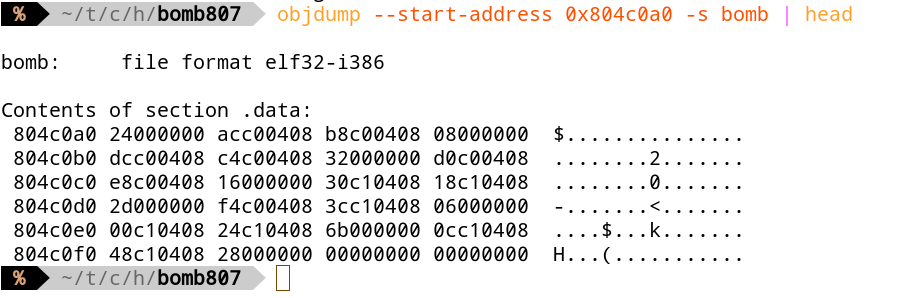
\includegraphics[width=0.95\linewidth]{resources/fig15.png}
			\caption{二叉树的反汇编部分}
			\label{fig:fig15}
		\end{figure}
	\item 对于反汇编的二叉树进行分析,可得二叉树的结构如图\ref{fig:fig16}所示。
		\begin{figure}[H]
			\centering
			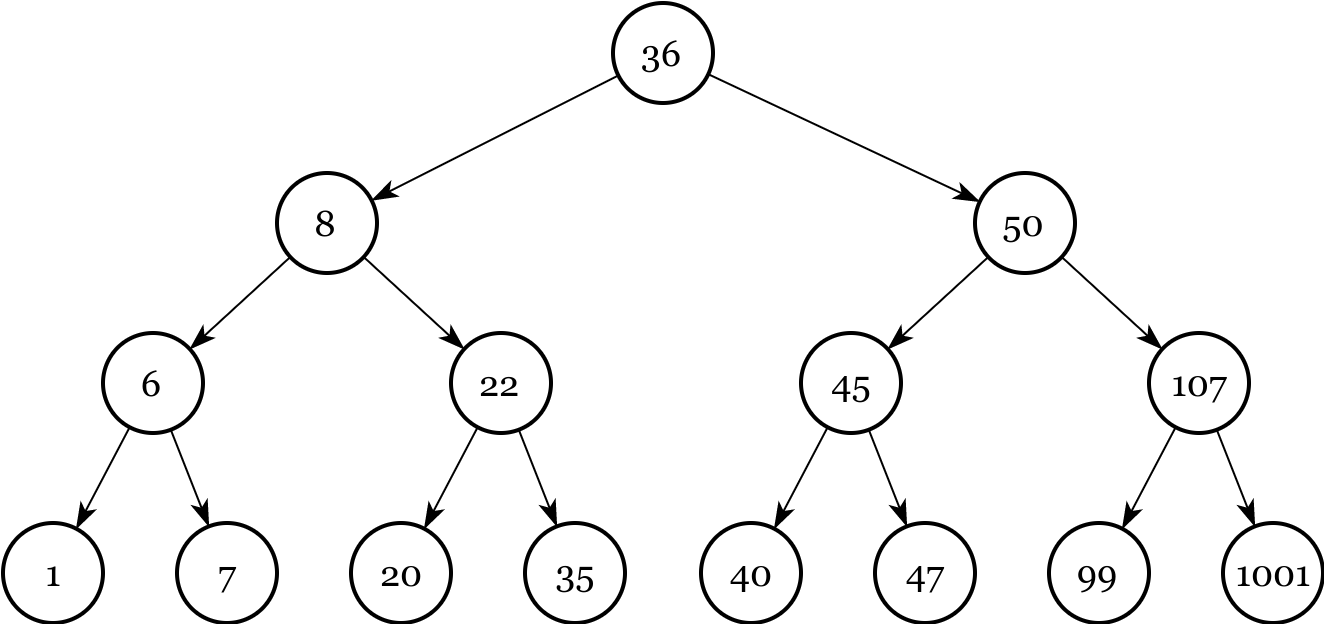
\includegraphics[width=0.95\linewidth]{resources/fig16.png}
			\caption{二叉树结构}
			\label{fig:fig16}
		\end{figure}
	\item 由图以及函数的调用规则可知,由于secrect\_phase中fun7的返回值为0,最后的答案为1或6或8或36。
	\item 将1输入炸弹,成功拆除炸弹的隐藏部分,如图\ref{fig:fig17}所示。
		\begin{figure}[H]
			\centering
			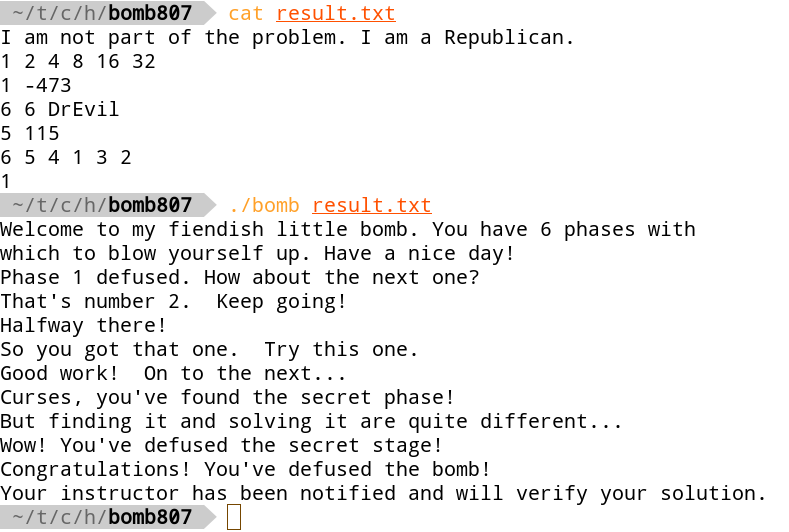
\includegraphics[width=0.95\linewidth]{resources/fig17.png}
			\caption{炸弹的隐藏部分的拆除}
			\label{fig:fig17}
		\end{figure}
\end{itemize}

\subsubsection{实验结果}
由实验过程可知,隐藏阶段的入口为在第四阶段的答案后追加DrEvil,隐藏阶段的解为字符串``1''。

\section{实验小结}
通过本次实验,我对于汇编,以及C语言如何转换为汇编有了更深入的了解。尤其第第6阶段,综合了各方面的指示,让我对于二进制程序的结构有了更深入的了解。相较于第一次实验,第二次实验增加了一定的难度,也使用了部分逆向工程的知识,让我更加深刻的体会到了这门课的魅力。

\end{document}
